\documentclass[12pt,a4paper,oneside,DIV12]{scrreprt}

%%%%%%%%%%%%%%%%%%%%%%%%%%%%%%%%%%%%%%%%%%
%% Author, Title
%%%%%%%%%%%%%%%%%%%%%%%%%%%%%%%%%%%%%%%%%%
\newcommand{\myAuthor}{Michael Sams}
\newcommand{\myTitle}{BAT - Bolt Analysis Tool}

%%%%%%%%%%%%%%%%%%%%%%%%%%%%%%%%%%%%%%%%%%
%% Used packages
%%%%%%%%%%%%%%%%%%%%%%%%%%%%%%%%%%%%%%%%%%
\frenchspacing
\usepackage[utf8]{inputenc}
\usepackage[english]{babel}
\usepackage{amsmath,amssymb,amstext,bm}
\usepackage{graphicx}
\usepackage{graphics}
\usepackage{geometry}
\graphicspath{{pictures/}}
\usepackage{listings}
\usepackage{units}
\usepackage[T1]{fontenc}
\usepackage{threeparttable}
\usepackage{wasysym}
\usepackage[final]{pdfpages}
\usepackage{lmodern}
\usepackage{courier}
\usepackage[    pdfauthor={\myAuthor},
                pdftitle={\myTitle},
                colorlinks=true,
                linkcolor=black,
                citecolor=black,
                urlcolor=black]{hyperref}
\usepackage{bibgerm}
% packages for pseudocode
\usepackage{algorithm}
\usepackage{algorithmic}
\renewcommand{\algorithmiccomment}[1]{{\color{gray}  // \textit{#1}}}
\usepackage{setspace}
\usepackage{xcolor}
\definecolor{light-gray}{gray}{0.95}
% subfigure
\usepackage[hang]{subfigure}
\usepackage{rotating}
% packages for definitions
\usepackage{shadethm}
% Tables
\usepackage{longtable,lscape}
\usepackage{setspace} %Fußnoten in Tabellen
\usepackage{threeparttable} %Fußnoten in Tabellen
\usepackage{multirow}
\usepackage{tabularx}
\usepackage{booktabs} %JCUmgebung für Tabellen in Wissenschaftlichen Publikationen
\usepackage{paralist}
\usepackage{array}
\usepackage{footnote}
\makesavenoteenv{table}
% multicolumn
\usepackage{multicol}

%%%%%%%%%%%%%%%%%%%%%%%%%%%%%%%%%%%%%%%%%%
%% Definitions 
%%%%%%%%%%%%%%%%%%%%%%%%%%%%%%%%%%%%%%%%%%
% theorem / definition
\newshadetheorem{definitions}{Definition}%[section]
\newenvironment{definition}[1][]{
  \definecolor{shadethmcolor}{rgb}{0.9,0.9,0.9}
  %\definecolor{shaderulecolor}{rgb}{0.0,0.0,0.4}
  %\setlength{\shadeboxrule}{1.5pt}
  \begin{definitions}[#1]\hspace*{1mm}
}{\end{definitions}}
\newshadetheorem{theorems}{Theorem}%[section]
\newenvironment{theorem}[1][]{
  \definecolor{shadethmcolor}{rgb}{0.9,0.9,0.9}
  %\definecolor{shaderulecolor}{rgb}{0.0,0.0,0.4}
  %\setlength{\shadeboxrule}{1.5pt}
  \begin{theorems}[#1]\hspace*{1mm}
}{\end{theorems}}
% command-definitions 
\newcommand{\sspace}{\mathcal{S}}
\newcommand{\real}{\mathbb{R}}
\newcommand{\expec}[2]{\mathbb{E}_{#2}[#1]}
\newcommand{\entropy}[1]{\mathbb{H}[#1]}
\newcommand{\expecij}[1]{\underset{i\neq j}{\mathbb{E}}[#1]}
\newcommand{\expecijm}[2]{\underset{i\neq #1}{\mathbb{E}}[#2]}
\newcommand{\vari}[1]{\text{var}[#1]}
\newcommand{\covari}[2]{\text{cov}[#1,#2]}
\newcommand{\kl}[2]{\text{KL}(#1||#2)}
\newcommand{\lowbound}[1]{\mathcal{L}(#1)}

% Abbreviations
\usepackage[printonlyused]{acronym}

% Footnote numbering
\usepackage{chngcntr}
\counterwithout{footnote}{chapter}

% Seitenumbruch: Verhindert Hurenkinder und Schusterjungen voellig
\widowpenalty=10000
\clubpenalty=10000
\displaywidowpenalty=10000

% caption of figures
\usepackage{caption}
\renewcommand{\capfont}{\footnotesize}
\renewcommand{\caplabelfont}{\footnotesize\bfseries}

%%%%%%%%%%%%%%%%%%%%%%%%%%%%%%%%%%%%%%%%%%
% Hyphenation
%%%%%%%%%%%%%%%%%%%%%%%%%%%%%%%%%%%%%%%%%%
%\hyphenation{Ver-sag-ens-kri-ter-ium}
%%%%%%%%%%%%%%%%%%%%%%%%%%%%%%%%%%%%%%%%%%

\begin{document}
% shortcuts for ref
%\newcommand{\equ}[1]{Equ.~\ref{#1}}
\newcommand{\equ}[1]{(\ref{#1})}
\newcommand{\defi}[1] {{\small\textsf{Definition~\ref{#1}}}}
\newcommand{\chapt}[1]{{\small\textsf{Chapter~\ref{#1}}}}
\newcommand{\sect}[1] {{\small\textsf{Section~\ref{#1}}}}
\newcommand{\fig}[1]  {{\small\textsf{Figure~\ref{#1}}}}
\newcommand{\alg}[1]  {{\small\textsf{Algorithm~\ref{#1}}}}
\newcommand{\tab}[1]  {{\small\textsf{Table~\ref{#1}}}}
\newcommand{\myspacing}{1.0}
\newcommand{\myfontsize}{10}
\newcommand{\myfontskip}{17}

\pagenumbering{roman}

%% title page 
\begin{titlepage}
  \newgeometry{left=35mm, right=35mm, top=25mm, bottom=15mm}

  %\begin{figure}
  %  \centering 
  %  \subfigure{\includegraphics[width=0.25\textwidth]{lnm_logo_01.png}}
  %  \hspace{6cm}
  %  \subfigure{\includegraphics[width=0.3\textwidth]{tum_logo_pdf2.pdf}}
  %\end{figure}

\vspace*{0.1cm}
\begin{center}

  \Huge{\normalfont{\sffamily{\bfseries{\myTitle}}}}\\

  \vspace{1.0cm}

  \begin{figure}[!htpb]
    \centering
    
\includegraphics[width=0.4\textwidth]{logo_try.png}
  \end{figure}
 
  \vspace{1.0cm}
 
  \Large{\textbf{User Manual}}
\end{center}

\vspace{2.5cm}

\begin{tabularx}{\textwidth}{ll}
\toprule
Author:    & \myAuthor \\
Issue:     & 0.2 \\
Date:      & \today \\
\bottomrule
\end{tabularx}

\end{titlepage}

%\thispagestyle{empty}   % nichts auf der Seite
%\mbox{}\cleardoublepage % leere Seite

%% table of contents
\tableofcontents

%% symbols and abbreviations 
\chapter*{Symbols and Abbreviations}

\subsubsection*{Symbols}
\begin{longtable}{p{2cm} l}
  $\alpha_A$ & tightening factor (assembly uncertainty factor)\\
  $\alpha_b$ & coefficient of linear thermal expansion of the bolt \\
  $\alpha_{ci}$ & coefficient of linear thermal expansion of the clamped part $i$ \\
  $\delta_b$ & elastic compliance of the bolt \\
  $\delta_c$ & elastic compliance of the clamped part (plate) \\
  $\varepsilon_{th}$ & linear thermal elongation \\
  $\theta$ & half angle of thread groves \\
  $\varkappa$ & parameter for elastic or plastic shear stress behaviour \\
  $\lambda$ & under-head bearing angle of bolt \\
  $\mu_T$ & coefficient of friction in the clamped part interfaces \\
  $\mu_{th}$ & coefficient of friction in bolt thread \\
  $\mu_{uh}$ & coefficient of friction under bolt head \\
  $\nu$ & bolt utilization factor \\
  $\varphi$ & helix angle / slope of bolt thread \\
  $\varphi_c$ & compression cone half angle \\
  $\Phi$ & load factor of concentric joint \\
         & (also: force ratio or relative compliance factor) \\
  $\Phi_n$ & load factor for concentric clamping and concentric \\
           & force load introduction via the clamped parts \\
  $\rho$ & friction angle in bolt thread \\
  $\sigma_M$ & normal stress in the bolt at $F_M$ \\
  $\sigma_{v,M}$ & von-Mises equivalent stress in the bolt at $F_M$ \\
  $\sigma_u$ & material ultimate strength \\
  $\sigma_y$ & material yield strength \\
  $\tau_M$ & shear stress in the bolt at $F_M$\\
  & \\
  $A_0$ & relevant stress cross section (BAT: $A_0 = A_s$) \\
  $A_1$ & nominal cross section of threaded bolt \\
  $A_3$ & minimal thread cross section \\
  $A_i$ & cross sectional area of component / segment $i$ \\
  $A_p$ & pitch cross section of threaded bolt \\
  $A_s$ & stress cross section of threaded bolt \\
  $A_{sub}$ & substitutional compliance area (BAT specific) \\
  $c$ & stiffness \\
  $c_b$ & bolt stiffness \\
  $c_c$ & clamp part stiffness \\
  $d$ & nominal threaded bolt diameter \\
  $d_0$ & relevant stress diameter (BAT: $d_0=d_s$) \\
  $d_2$ & pitch diameter of threaded bolt \\
  $d_3$ & minimal diameter of threaded bolt \\
  $d_h$ & minimal contact diameter under bolt head \\
  $d_s$ & stress diameter of threaded bolt \\
  $D_{avail}$ & available diamter for compression zone \\
  $D_{hole}$ & through-hole diameter (drilled bolt hole) \\
  $D_{Km}$ & effective diameter of under head/nut friction torque \\
  $D_{lim}$ & limiting diameter of compression zone \\
  $E_b$ & Young's Modulus of bolt \\
  $E_c$ & Young's Modulus of clamped part \\
  $F_A$ & external, axial bolt load \\
  $F_K$ & clamp load \\
  $F_{KR}$ & residual clamp load at the interface during loading in service \\
  $F_{Kreq}$ & required clamping force for friction grip per bolt \\
  $F_M$ & preload after tightening / assembly preload \\
  $f_P$ & clamped part compression \\
  $f_{PA}$ & additional deformation of clamped part due to loading \\
  $F_{PA}$ & additional axial plate load \\
  $F_Q$ & external, shear bolt load \\
  $f_S$ & bolt elongation \\
  $F_S$ & bolt load \\
  $f_{SA}$ & additional elongation of bolt due to loading \\
  $F_{SA}$ & additional axial bolt load \\
  $\Delta F_{Vth}$ & thermal preload change \\
  $F_V$ & service preload incl. embedding and thermal influence \\
  $f_Z$ & plastic deformation due to embeddding \\
  $F_Z$ & preload loss due to embedding \\
  $K$ & joint coefficient \\
  $k_{\tau}$ & shear stress reduction coefficient \\
  $L_i$ & length of component/segment $i$ \\
  $\Delta L$ & total change in length after temperature loading (bolt and clamped parts) \\
  $\Delta l_b$ & change in length of bolt after temperature loading \\
  $l_{0b}$ & initial length of bolt ($=l_K$) without temperature loading \\
  $\Delta l_c$ & change in clamped part thickness after temperature loading \\
  $l_{ci}$ & thickness of clamp part $i$ \\
  $l_{0ci}$ & initial thickness of clamp part $i$ without temperature loading \\
  $L_{eng,sub}$ & substitutional length of engaged thread \\
  $L_{h,sub}$ & substitutional length of bolt head \\
  $l_K$ & joint clamped length \\
  $L_{n,sub}$ & substitutional length of nut (locking device) \\
  $M_{th}$ & friction torque at thread interface \\
  $M_p$ & prevailing torque of bolt locking device \\
  $M_{uh}$ & under-head torque due to friction \\
  $n$ & loading plane factor / load introduction factor \\
  $p$ & pitch of bolt thread \\
  $q_F$ & number of shear force transmitting interfaces \\
  $\Delta T$ & temperature gradient \\
  $T_A$ & total installation torque of bolt \\
  $T_{scatter}$ & torque scatter of tightening device (torque wrench) \\
  $W_p$ & polar section modulus / polar moment of resistance \\
  $w$ & parameter for $\delta_c$ calculation (TBJ: $w=1$, TTJ: $w=2$) \\
  $x$ & first parameter for $\varphi_c$ calculation \\
  $x_c$ & parameter for $\delta_c$ calculation for multiple clamped parts (BAT specific) \\
  $y$ & second parameter for $\varphi_c$ calculation \\
\end{longtable}

\subsubsection*{Abbreviations}
\begin{tabular}{p{3cm} l}
  BAT & Bolt Analysis Tool \\
  CTE & Coefficient of Thermal Expansion \\
  MOS & Margin of Safety \\
  TBJ & Through-Bolt Joint \\
  TTJ & Tapped Thread Joint \\
\end{tabular}
%\mbox{}\cleardoublepage % leere Seite

%% figure and tab-list
%\chapter*{List of figures, tables and algorithms}


%\subsection*{Figures}
%\begingroup % group, damit kein Seitenumbruch entsteht
%  \renewcommand\listfigurename{}
%  \let\clearpage\relax
  %\listoffigures
%\endgroup

%\subsubsection*{Tables}
%\addtocontents{lof}{\vskip -1.2cm}
%\begingroup % group, damit kein Seitenumbruch entsteht
%  \renewcommand\listtablename{}
%  \let\clearpage\relax
  %\listoftables
%\endgroup

{ \listoffigures
    \let\clearpage\relax
  \listoftables
    \let\clearpage\relax
  \listofalgorithms
}


\setcounter{page}{1}
\pagenumbering{arabic}
%% Chapters
\chapter{Introduction}
This document will include the \textbf{BAT} (Bolt Analysis Tool) User Manual.
\begin{colbox}{BAT Info:}
  The current design status of the \emph{Bolt Analysis Tool} \textbf{BAT} only includes 
  \emph{Concentric Axially Loaded Bolted Joints}. 
\end{colbox}

\chapter{Bolt and Thread Geometry}
$D_{Km}$ is the \emph{effective diameter of under head/nut friction torque} and is defined by 
\begin{equation}
  D_{Km} = \frac{D_{hole}+d_h}{2}
  \label{equ:dkm}
\end{equation}
where $D_{hole}$ is the \emph{through-hole diameter} in the clamped parts and $d_h$ is the 
\emph{minimum bearing surface outer diamter} of the bolt head or nut. An other input value to calculate
the under-head friction torque \equ{equ:Muh} is the \emph{under head bearing angle} $\lambda$ seen in 
\fig{fig:ecss_uh_brg_angle}.
\begin{figure}[!htpb]
  \centering
  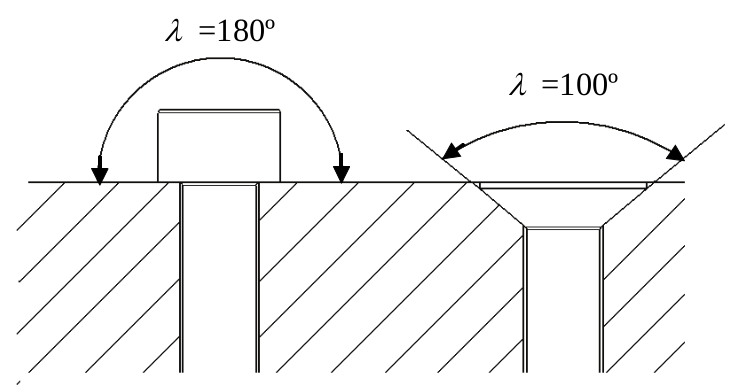
\includegraphics[width=0.5\textwidth]{ECSS_uh_brg_angle.png}
  \caption{Definition of under head bearing angle \cite{ECSS_HB_32_23A}}
  \label{fig:ecss_uh_brg_angle}
\end{figure}

\chapter{Joint Diagram}
\label{ch:jointdiag}
The \emph{joint diagram} seen in \fig{fig:joint_diagram} \cite{VDI2230_1} visualizes the forces and 
displacements and helps to understand the loading conditions of a concentrically loaded bolted joint. 
\begin{figure}[!htbp]
  \centering
  \subfigure[without loading plane effect $n=1$ \cite{VDI2230_1}]{
    \label{fig:joint_diagram}
    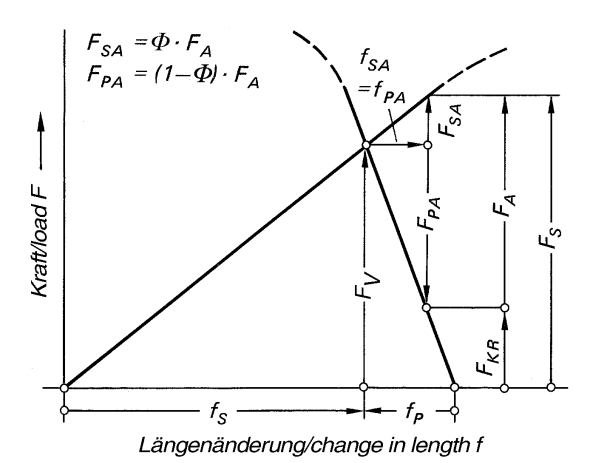
\includegraphics[width=0.43\textwidth]{VDI2230_Bild24.png}
  }
  \subfigure[with loading plane effect $n<1$ \cite{ESAPSS}]{
    \label{fig:joint_diagram_n}
    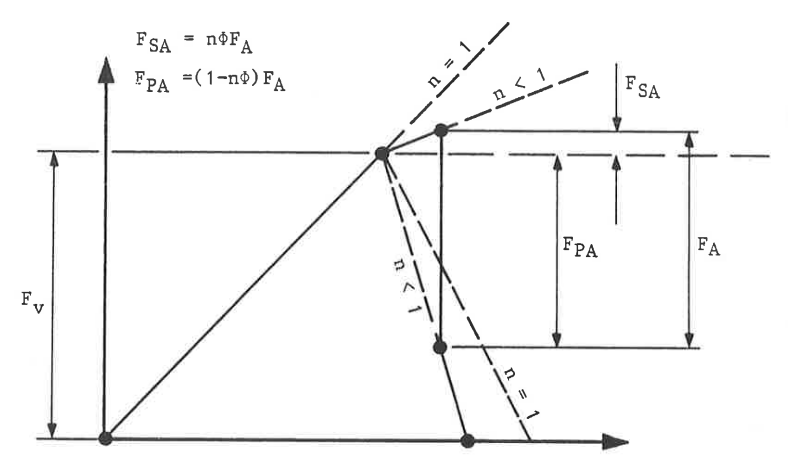
\includegraphics[width=0.52\textwidth]{ESAPSS_joint_diagram_loading_loading_plane.png}
  }
  \caption{Joint diagram for the working state of a concentrically loaded bolted joint}
\end{figure}

The preload force $F_V$ (see §\ref{sec:preload}) compresses the clamped parts $f_P$ and elongates
the bolt $f_S$ during tightening. If an external load $F_A$ is acting on the bolted joint the bolt
is streched much further and the clamped parts are relaxed ($f_{SA}=f_{PA}$) due to the loading. 
The \emph{additional axial bolt load} $F_{SA}$ and the \emph{additional axial plate load}\footnotemark[1]
\footnotetext[1]{If the bolt is loaded in tension $F_{PA}$ is better described as an 
\emph{axial plate relaxation force}.} $F_{PA}$ are given to
\begin{equation}
  F_{SA} = n \Phi F_A, \qquad F_{PA} = (1-n \Phi) F_A
  \label{equ:FSA_FPA}
\end{equation}
where $\Phi$ is the load factor, which is defined as the quotient of the additional bolt load $F_{SA}$ 
and the axial working load component $F_A$. $n$ is the \emph{loading plane factor} and is crucial
for determining the size of the additional bolt loads. As seen in \fig{fig:joint_diagram} $F_{KR}$ is the residual
clamping load at the interface during relief or loading by $F_{PA}$ and after embedding in service and 
$F_S$ is the maximum bolt load. 
\section{Loading Plane Factor}
A simple explanation of the \emph{loading plane effect} is given in \cite{ESAPSS} and this text is 
used directly for the description in this document. 

\fig{fig:esapss_lpf_1} shows the external load applied at planes under the bolt head and under the nut. 
The extreme case where the external bolt force $F_A$ is acting directly under head / nut is rare
($n=1$), usually the effective loading planes are considered to be within the joint as seen in 
\fig{fig:esapss_lpf_1}, $n l_K$ apart ($n<1$). 

Between the loading planes the joint is reliefed by $F_A$ but outside of the loading planes the clamped
material is subjected to $F_A$ in addition to $F_K$ the clamping load. The effect of this to the loading 
diagram is shown in \fig{fig:joint_diagram_n}. The effective bolt stiffness is reduced and the 
effective joint stiffness increased as $n$ reduces. Hence the closer the load application is to the 
joint interface the smaller is the external force seen by the bolt $F_{SA}$. 

For a more detailed explanation of the \emph{loading plane factor} and for the correct derivation
and analysis of $n$ see \cite{VDI2230_1,ECSS_HB_32_23A}.
\begin{figure}[!htpb]
  \centering
  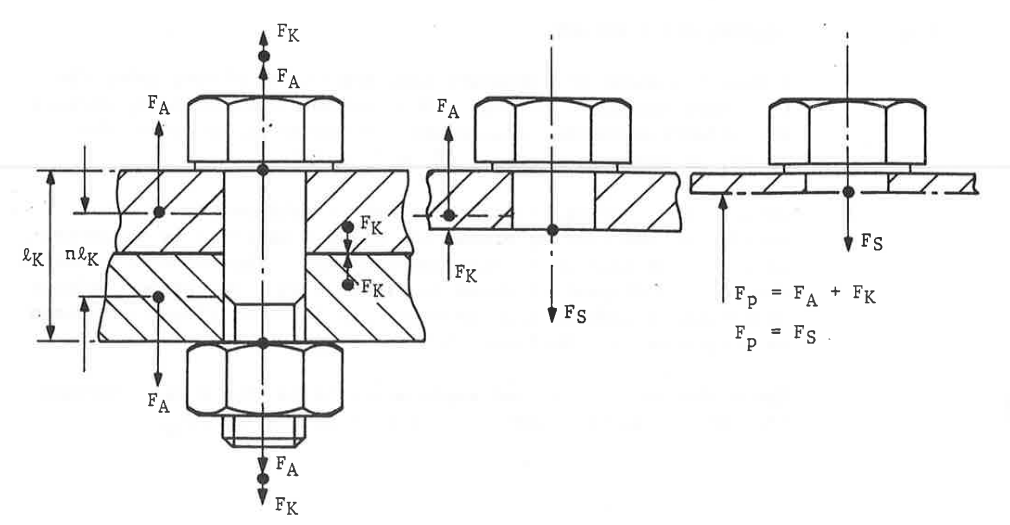
\includegraphics[width=0.99\textwidth]{ESAPSS_loading_plane_factor.png}
  \caption{Tension joint loading planes and the forces acting within the joint \cite{ESAPSS}}
  \label{fig:esapss_lpf_1}
\end{figure}
\begin{colbox}{Approximate Method \cite{ECSS_HB_32_23A}:}
  The loading plane factor depends on the deformation of the joint caused by preload. For uncritical
  verification purposes with simple joint geometry the loading plane factor may be set to $n=0.5$,
  which assumes that the loading planes are at the center of each flange.
\end{colbox}

\chapter{Method B: ECSS-E-HB-32-23A}
This chapter provides a quick overview and summary of the equations used in \bat. A detailed description
can be found in the complete ECSS-E-HB-32-23A ESA handbook \cite{ECSS_HB_32_23A}. Some used variables
in the following equations have been changed compared to \cite{ECSS_HB_32_23A} by the author to increase
clarity and consistency.

\section{Preload and Torques}
\label{sec:preload}
The torque present at the thread interface $M_{th}$ is dependent of the \emph{axial bolt preload} $F_V$ 
and is given by
\begin{equation}
  M_{th} = F_V \tan(\varphi+\rho)\frac{d_2}{2}
  \label{equ:M_th}
\end{equation}
and the \emph{under-head torque} $M_{uh}$ due to friction between bolt head or nut and the adjacent 
clamped part (or shim) is defined by
\begin{equation}
  M_{uh} = F_V \frac{\mu_{uh} D_{Km}}{2} \frac{1}{\sin{\nicefrac{\lambda}{2}}}
  \label{equ:Muh}
\end{equation}
where $\lambda$ is the \emph{under head bearing angle} seen in \fig{fig:ecss_uh_brg_angle}.
It is assumed that the friction force for $M_{uh}$ is acting at mean bearing radius of the bolt head 
$D_{Km}$ \equ{equ:dkm}. $\varphi$ is the helix angle of the thread and $\rho$ is given by the relation
\begin{equation}
  \tan\rho = \frac{\mu_{th}}{\cos\nicefrac{\theta}{2}}
\end{equation}
where $\theta$ is the half angle of the thread groves (for Unified or Metric threads $\theta=60^\circ$).

The \emph{total installation torque} $T_A$ (without torque device scatter) applied to bolt head or nut
during tightening to produce the axial bolt preload $F_V$ is 
\begin{equation}
  T_A = M_{th} + M_{uh} + M_p
  \label{equ:TA}
\end{equation}
where $M_p$ is the \emph{prevailing torque} of the locking device. 
With the approximation $\tan\varphi \tan\rho \ll 1$ the expression $\tan(\varphi+\rho)$ can be written
as $\tan(\varphi+\rho) \approx \tan\varphi + \tan\rho$. Now equation \equ{equ:TA} can be rewritten to
\begin{equation}
  T_A = F_V \underbrace{ \left[ \frac{d_2}{2} \left( \tan\varphi + \frac{\mu_{th}}{\cos\nicefrac{\theta}{2}} \right) 
  + \frac{\mu_{uh} D_{Km}}{2 \sin\nicefrac{\lambda}{2}} \right]}_{K} + M_p
  \label{equ:TA2}
\end{equation}
where $K$ is the \emph{joint coefficient}.

\begin{colbox}{BAT Info:}
  For calculation of the minimum and maximum axial bolt preload, BAT implements the 
  \emph{experimental coefficient method} \cite{ECSS_HB_32_23A} with an explicit torque scatter torque
  of the tightening device $T_{scatter}$.
\end{colbox}
The minimum and maximum total installation torques with included torque scatter are defined 
\begin{equation}
  T_A^{min} = T_A - T_{scatter} , \qquad T_A^{max} = T_A + T_{scatter}.
  \label{equ:Tscatter}
\end{equation}
To calculate the minimum and maximum \emph{axial bolt preload after tightening} $F_M^{min/max}$, 
\equ{equ:TA2} and \equ{equ:Tscatter} are combined 
\begin{equation}
  F_M^{min} = \frac{T_A^{min}-M_p^{max}}{K^{max}} ,\qquad
  F_M^{max} = \frac{T_A^{max}-M_p^{min}}{K^{min}}.
\end{equation}
If also the thermal influence and embedding is considered, this leads to the minimum and maximum
\emph{axial bolt preload at service} $F_V^{min/max}$
\begin{subequations}
  \setlength{\jot}{10pt}
  \begin{align}
    F_V^{min} &= \frac{T_A^{min}-M_p^{max}}{K^{max}}+\Delta F_{Vth}-F_Z \\
    F_V^{min} &= F_M^{min}+\Delta F_{Vth}-F_Z \\
    &= \frac{T_A^{min}-M_p^{max}}{\frac{d_2}{2} \left( \tan\varphi + \frac{\mu_{th}^{max}}
    {\cos\nicefrac{\theta}{2}} \right) + \frac{\mu_{uh}^{max} D_{Km}}
    {2 \sin\nicefrac{\lambda}{2}}}+\Delta F_{Vth}-F_Z
    \label{equ:FVmin}
  \end{align}
\end{subequations}
\begin{subequations}
  \setlength{\jot}{10pt}
  \begin{align}
    F_V^{max} &= \frac{T_A^{max}-M_p^{min}}{K^{min}}+\Delta F_{Vth} \\
    F_V^{max} &= F_M^{max}+\Delta F_{Vth} \\
    &= \frac{T_A^{max}-M_p^{min}}{\frac{d_2}{2} \left( \tan\varphi + \frac{\mu_{th}^{min}}
    {\cos \nicefrac{\theta}{2}} \right) + \frac{\mu_{uh}^{min} D_{Km}}
    {2 \sin \nicefrac{\lambda}{2}}}+\Delta F_{Vth}
    \label{equ:FVmax}
  \end{align}
\end{subequations}
where $\Delta F_{Vth}$ is thermal preload change (see §\ref{sec:thermal}) and 
$F_Z$ is the preload loss due to embedding (see §\ref{sec:embedding}).

The tightening factor $\alpha_A$ (assembly uncertainty factor) which takes into account the scatter 
of the achievable assembly preload between $F_M^{max}$ and $F_M^{min}$ is introduced in the following form 
\begin{equation}
  \alpha_A = \frac{F_M^{max}}{F_M^{min}}
\end{equation}

\section{Thermal Influcence}
\label{sec:thermal}
If a thermal load is applied to a bolted joint, the bolt sees a change $\Delta F_{Vth}$ in the preload
force due to the CTE mismatch of bolt and clamped parts seen in \equ{equ:FVmin} and \equ{equ:FVmax}.
\subsection{Linear Thermal Influence}
For the following derivation it is assumed that the Young's Modulus $E$ of bolt and clamped parts does 
not change with temperature (temperature independent material properties). $c_b=\nicefrac{1}{\delta_b}$
and $c_c=\nicefrac{1}{\delta_c}$ are defined as bolt stiffness and clamp-part stiffness respectively.
Linear thermal elongation is defined
\begin{equation*}
  \varepsilon_{th} = \alpha \Delta T = \frac{\Delta l}{l_0}
\end{equation*}
The thermal elongation for bolt (index $b$) and clamped-parts (index $c$) are given to
\begin{subequations}
  \begin{align*}
    \Delta l_b &= \alpha_b \cdot \Delta T \cdot l_{0b} \\
    \Delta l_c &= \sum_i \alpha_{ci} \cdot \Delta T \cdot l_{0ci}
  \end{align*}
\end{subequations}
where $l_K = l_{0b} = \sum_i l_{0ci}$ is the clamping length of the joint.
\begin{colbox}{BAT Info:}
  The sign definition in BAT is $\Delta L = \Delta l_c - \Delta l_b$ and this leads to 
  \begin{subequations}
    \begin{align*}
      \alpha_c > \alpha_b &\Rightarrow \pmb{+}\Delta F_{Vth} \\
      \alpha_c < \alpha_b &\Rightarrow \pmb{-}\Delta F_{Vth}
    \end{align*}
  \end{subequations}
  where $\pmb{+}\Delta F_{Vth}$ defines an increase and $\pmb{-}\Delta F_{Vth}$ a loss in bolt preload.
\end{colbox}
If the standard stiffness equation $F=c \cdot \Delta x$ is used for the bolt / clamp-part joint, this leads to
\begin{subequations}
  \setlength{\jot}{10pt}
  \begin{align}
    \Delta F_{Vth} &= c \cdot \Delta L \\
    &= \frac{\Delta L}{\frac{1}{c_b}+\frac{1}{c_c}} \\
    &= \Delta L \frac{c_b c_c}{c_b + c_c} = \Delta L \frac{1}{\delta_b + \delta_c}
    \label{equ:dFVth}
  \end{align}
\end{subequations}

\subsection{VDI Method}
to be filled

\section{Embedding}
\label{sec:embedding}
When bolts are first tightened the male and female thread, the under-head and under-nut surfaces and the 
clamped parts interface contact each other only on microscopically small high spots (surface roughness).
The material at these hight spots will be overloaded, well past their yield point, during initial 
tightening and will subsequently creep until a large enough area of the available contact surface has 
been engaged to stabilize the process. In addition, plastic flow will often occur at the highest stressed 
points such as thread roots or at the first engaged thread in the nut. These relatively short-term 
relaxation effects are known as \emph{embedding}. After tightening the rate of relaxation is a maximum, 
reducing exponentially, usually over the first few minutes, to a constant very low rate of creep. 
Typically embedding accounts for only a few percent loss of initial preload, however $5\%$ to $10\%$ are
not uncommon \cite{ECSS_HB_32_23A}. The value significantly depends on the amount and hardness of the 
clamping parts. 

The \emph{embedding preload loss} $F_Z$ depends on the plastic deformation $f_Z$ of the joint.
\begin{equation*}
  \frac{F_Z}{F_V}=\frac{f_Z}{\left(\delta_b+\delta_c\right)F_V}
\end{equation*}
This it follows that, 
\begin{equation}
  F_Z=\frac{f_Z}{\delta_b+\delta_c}
\end{equation}
where $f_Z$ depends on surface roughness, the number of clamped parts interfaces in the joint and the 
material type (and hardness). For uncritical cases a value of $5\%$ of the preload can be used for 
calculation purposes \cite{ECSS_HB_32_23A}.
\begin{colbox}{BAT Info:}
  In BAT, the $5\%$ embedding preload loss is defined for the maximum bolt preload after tightening.
  \begin{equation*}
    F_Z = 0.05 F_M^{max}
  \end{equation*}
\end{colbox}
It is always recommended that the correct embedding preload loss is determined by experiment. If no 
experimental data is available \tab{tab:vdi_embedding} can be used to find approximate values. 
This table may only be used if the service temperatures are below $50\%$ of the recrystallization
temperatures of the used materials. The table used in ECSS-E-HB-32-23A \cite{ECSS_HB_32_23A} is used 
out of the VDI 2230 guideline \cite{VDI2230_1}. 
\begin{table}[!htpb]
  \centering
  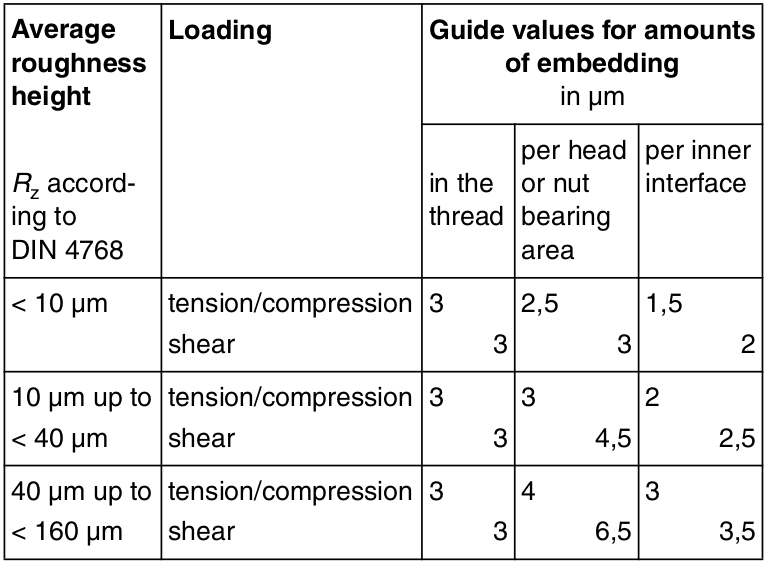
\includegraphics[width=0.5\textwidth]{VDI2230_embedding.png}
  \caption{Guide values for amounts of embedding of bolts, nuts and compact clamped parts made of steel, without coatings \cite{VDI2230_1}}
  \label{tab:vdi_embedding}
\end{table}
\begin{colbox}{BAT Info:}
  Only the maximum embedding values listed in \tab{tab:vdi_embedding} for tension/compression and shear 
  are used in BAT (no distinction between external loading types).
\end{colbox}

\section{Compliance of Bolt and Clamped Parts}
\subsection{Compliance of Bolt}
\label{ssec:compl_bolts}
The bolt consists of different sections with dedicated compliances seen in \fig{fig:ECSS_bolt_compliance}.
\begin{figure}[!htpb]
  \centering
  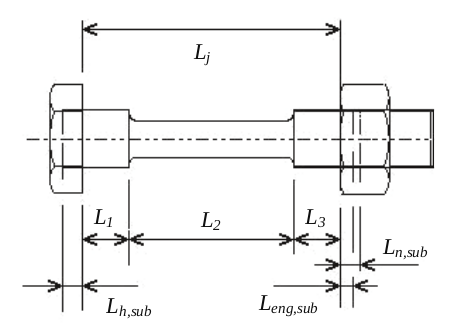
\includegraphics[width=0.5\textwidth]{ECSS_bolt_compliance.png}
  \caption{Dimensioning of the bolt for compliance calculation \cite{ECSS_HB_32_23A}}
  \label{fig:ECSS_bolt_compliance}
\end{figure}

Applying the Hook's law to each segment of the bolt and combining the equations, the compliance of the 
bolt $\delta_b$ can be written
\begin{equation}
  \delta_b = \frac{1}{c_b}=\frac{1}{E_b}\sum\frac{L_i}{A_i}
  \label{equ:delta_b_1}
\end{equation}
where $c_b=\nicefrac{1}{\delta_b}$ is the bolt stiffness, $A_i$ and $L_i$ are the segment cross section 
and segement lengths respectively. $E_b$ is the bolt Young's Modulus and 
$A_i$ are the cross sections for each bolt segement. Expanding \equ{equ:delta_b_1} and introducing 
substitution lengths for deformation in the bolt head and engaged region in thread and nut the equation
leads to
\begin{equation}
  \delta_b = \frac{1}{E_b}\left[\frac{L_{h,sub}}{A_1}+\frac{L_{eng,sub}}{A_3}+\left(
    \frac{L_1}{A_{L_1}}+\frac{L_2}{A_{L_2}}+\dots+\frac{L_i}{A_{L_i}}\right)\right]
    +\frac{L_{n,sub}}{E_n A_1}
\end{equation}
where $L_{h,sub}$ and $L_{n,sub}$ are substitutional lengths of bolt head and nut (locking device) 
respectively. $L_{eng,sub}$ is the substitution length for the engaged thread and the value depends 
on the type of joint. For through bolt joint (TBJ) $L_{eng,sub}^{TBJ}=0.4d$ and for tapped thread 
joints (TTJ) $L_{eng,sub}^{TTJ}=0.33d$.
\begin{colbox}{BAT Info:}
  The current BAT implementation does not include \emph{shank bolts} with different diameter sections; 
  complete shaft length is threaded ($\sum \nicefrac{L_i}{A_i} = \nicefrac{l_K}{A_3}$). Also for the bolt head compliance only cylindrical
  head is considered $L_{h,sub}=0.4d$ for simplicity. The same substitution length is used for the
  locking device (nut) $L_{n,sub}=0.4d$ according to \cite{ECSS_HB_32_23A}. It is assumed that the nut
  has the same Young's Modulus than the bolt $E_n=E_b$. 
  \begin{subequations}
    \begin{align}
      \delta_b &= \frac{1}{E_b}\left(\frac{L_{h,sub}}{A_1}+\frac{L_{eng,sub}}{A_3}
        +\frac{L_i}{A_{L_i}}+\frac{L_{n,sub}}{A_1}\right) \\
        &= \frac{1}{E_b}\left(\frac{0.4d}{A_1}+\frac{L_{eng,sub}}{A_3}
        +\frac{l_K}{A_3}+\frac{0.4d}{A_1}\right)
    \end{align}
  \end{subequations}
\end{colbox}

\subsection{Compliance of Clamped Parts}
The calculation of the compliance of the clamped parts $\delta_c$ is more complicated than that of the 
bolts presented in §\ref{ssec:compl_bolts} because of the 3-dimensional stress state in the joint that 
is induced by the preload. The presented method \cite{ECSS_HB_32_23A} neglects the compliance of the 
interfaces and therefore it is most accurate for joints with a small number of clamped parts. If more
clamped parts are required the correct compliance can be determined by test or finite element analysis.

\begin{figure}[!htpb]
  \centering
  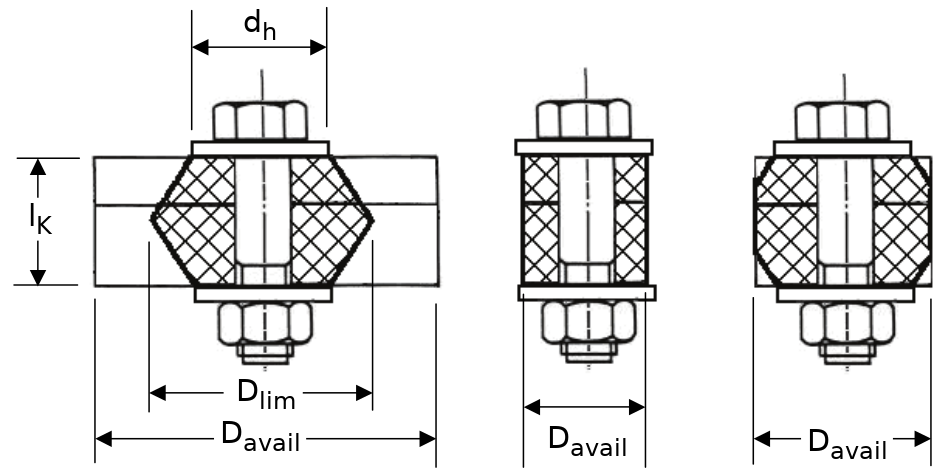
\includegraphics[width=0.9\textwidth]{ECSS_compr_zones_1.png}
  \caption{Compression zones in cylindrical clamped parts \cite{ECSS_HB_32_23A}}
  \label{fig:ECSS_compr_zones_1}
\end{figure}
The configuration of the \emph{compression zone} depends on the geometry of the clamped parts (joint
geometry). \fig{fig:ECSS_compr_zones_1} shows the three possible compression zones for cylindrical 
clamped parts\footnotemark[3]\footnotetext[3]{The figure assumes that the flanges are compressed
between infinitely stiff washers with the diameter equal to the \emph{minimal diameter under bolt
head} $d_h$ for the compression zone. In BAT the washer is considered as clamp part.}. 
The configuration on the left of \fig{fig:ECSS_compr_zones_1} has flanges that are sufficiently wide to
allow full spreading of the compression zone to the limiting diameter $D_{lim}$. In reality, the shape 
of the 3-dimensional zone of compression in an isotropic material is a paraboloid. The used 
approximate method simplifies the shape to a pair of compression cones. The two cones are symmetric 
about the mid-point of the clamped parts length $l_K$, which does not necessarily correspond to the 
interface between the flanges. If the flanges are too small for the compression cone to fully develop
$D_{avail}<D_{lim}$, a full or partial \emph{compression sleeve} develops. For \emph{tapped thread joints}
(TTJ) the analysis model assumes only one compression cone in the non-threaded clamped parts. 
For the general case with clamped parts that are not axially symmetric about the bolt axis, multiple 
edge distances are present; here the configuration of the deformation zone $D_{avail}^{min}$
should be determined by the minimum edge distance (inscribed diameter).
\subsubsection{Analysis Method}
If the edge distance of the flanges and hence the available diameter for the compression zone $D_{avail}$
is known, it can be compared with the \emph{limit diameter of the compression cone} $D_{lim}$, given by
\begin{equation}
  D_{lim} = d_h + w l_K \tan \varphi_c
\end{equation}
where $\varphi_c$ is the \emph{compression cone half angle} and the parameter $w$ is defined according
to the joint type. For through bolt joints $TBJ: w=1$ and for tapped thread joints $TTJ: w=2$. 
The compression cone half angle $\varphi_c$ can be derived with an empirical equation \cite{ECSS_HB_32_23A}
\begin{subequations}
  \begin{align}
    TBJ: \qquad \tan \varphi_c &= 0.362+0.032\ln\left(\nicefrac{x}{2}\right)+0.153\ln y \\
    TTJ: \qquad \tan \varphi_c &= 1.295-0.246\ln x +0.94\ln y
  \end{align}
\end{subequations}
where the following non-dimensional parameters are used $x=\nicefrac{l_K}{d_h}$, 
$y=\nicefrac{D_{avail}}{d_h}$. The existence of a compression sleeve is determined as follows:
\begin{description}
  \item[\textbf{CASE 1:} $\mathbf{D_{avail}>D_{lim}}$] the compression zone is fully developed into a cone or a pair 
    of cones for TBJ joints. The compliance of the clamped parts $\delta_c$ for a compression cone is given by 
    \begin{equation}
      \delta_c = \frac{2\ln\left[\frac{(d_h+d)(D_{lim}-d)}{(d_h-d)(D_{lim}+d)}\right]}
        {w E_c \pi d \tan \varphi_c}
      \label{equ:case_1}
    \end{equation}
  \item[\textbf{CASE 2:} $\mathbf{D_{avail}<d_h}$] only a compression sleeve and no compression cone
    develops due to small clamped part dimesions. The compliance of the clamped parts $\delta_c$ 
    for a compression sleeve is given by 
    \begin{equation}
      \delta_c = \frac{4 l_K}{E_c \pi \left( D_{avail}^2-d^2 \right)}
      \label{equ:case_2}
    \end{equation}
  \item[\textbf{CASE 3:} $\mathbf{d_h<D_{avail}<D_{lim}}$] partial compression sleeve and cone(s) develops.
    The compliance of the clamped parts $\delta_c$ for a combined cone / sleeve compression zone is given by 
    \begin{equation}
      \delta_c = \frac{\frac{2}{w d \tan \varphi_c}\ln\left[\frac{(d_h+d)(D_{avail}-d)}
        {(d_h-d)(D_{avail}+d)}\right] + \frac{4}{D_{avail}^2-d^2}\left[
          l_k - \frac{D_{avail}-d_h}{w \tan \varphi_c} \right]}{E_c \pi}
      \label{equ:case_3}
    \end{equation}
    This equation includes the effect of both the compression cone(s) and sleeve and is therefore 
    appropriate when the clamped parts have the same Young's Modulus. If the compliances of the cone and 
    sleeve should be calculated separately (multiple materials / different Young's Moduli present in the 
    clamped parts) the clamped part compliances should be calculated by a different method \cite{ECSS_HB_32_23A}
    $\rightarrow$ \textbf{OPEN ISSUE IN BAT - TO BE CHECKED}. 
\end{description}
\begin{colbox}{BAT Info:}
  Multiple clamped parts with different materials can be defined in BAT. To calculate the overall 
  clamped part compliance $\delta_c$ the equations described above for \emph{CASE 1, 2 and 3} are
  restructured. For each case a parameter $x_c$ is evaluated, which is simply the $\delta_c$-equations 
  \equ{equ:case_1}, \equ{equ:case_2} and \equ{equ:case_3} without the Young's Modulus $E_c$
  \begin{equation}
    \delta_c = \frac{l_K}{E_c A_{sub}}=\frac{x_c}{E_c} \qquad \rightarrow \qquad A_{sub}=\frac{l_K}{x_c}
  \end{equation}
  where $A_{sub}$ is the derived \emph{substitutional compliance area} of the clamped parts.
  It is assumed that $A_{sub}$ can be used to calculate the overall clamped part compliance for multiple 
  clamped parts with different Young's Moduli $E_{ci}$ and thicknesses $l_{ci}$
  \begin{equation}
    \delta_c = \frac{l_K}{\tilde{E_c} A_{sub}} = \sum_i \frac{l_{ci}}{E_{ci} A_{sub}}
  \end{equation}
\end{colbox}

\section{Stesses in Bolt and Clamped-Parts}
\subsection{Stress in bolt after tightening}
\label{ssec:stresses}
Based on §\ref{sec:preload} the stresses in the bolt after tightening can be derived. 
The minimum and maximum shear stress in the bolt $\tau_M^{min/max}$ after tightening can be calculated
as follows
\begin{equation}
  \tau_M^{min} = \frac{T_A^{min}-M_{uh}^{max}}{W_p} , \qquad \tau_M^{max} = \frac{T_A^{max}-M_{uh}^{min}}{W_p}
  \label{equ:tau_M}
\end{equation}
where $T_A$ is defined in \equ{equ:Tscatter}, $M_{uh}$ in \equ{equ:Muh} with $F_V=F_M$ and 
$W_p = \nicefrac{\pi d_s^3}{16}$ is the polar section modulus. The minimum and maximum normal 
stress $\sigma_M^{min/max}$ in the bolt caused by the preload is defined
\begin{equation}
  \sigma_M^{min/max} = \frac{F_M^{min/max}}{A_s}
  \label{equ:sig_M}
\end{equation}
The minimum and maximum von-Mises equivalent stress $\sigma_{v,M}^{min/max}$ in the bolt after tightening
(with $100\%$ shear stress contribution / $0\%$ shear stress relaxation) is defined 
\begin{equation}
  \sigma_{v,M}^{min/max} = \sqrt{\left(\sigma_M^{min/max}\right)^2 + 3\left(\tau_M^{min/max}\right)^2}
  \label{equ:sig_vM}
\end{equation}
Based on the von-Mises equivalent stress in the bolt the minimum and maximum 
\emph{bolt utilization} $\nu^{min/max}$ is defined
\begin{equation}
  \nu^{min/max} = \frac{\sigma_{v,M}^{min/max}}{\sigma_y}
  \label{equ:nu}
\end{equation}
where $\sigma_y$ is the bolt material yield strength and this defines the tightening status of the joint. 

\subsection{Stress and margins of safety in bolt at service}
The bolted joint can be loaded with an axial force $F_A$ and a shear force $F_Q$. For
the axial loading the additional bolt load is defined in \equ{equ:FSA_FPA} and for the shar loading
the required clamping force for friction grip per bolt is defined 
\begin{equation}
  F_{Kreq} = \frac{F_Q}{q_F \mu_T}
\end{equation}
where $q_F$ is the number of shear force transmitting interfaces and $\mu_T$ the coefficient of 
friction in the clamped part interfaces. 
\subsubsection{Local Slippage Margin $MOS_{slip}^{local}$}
The \emph{local slippage margin} is defined for a minimum preload $F_V^{min}$
\begin{equation}
  MOS_{slip}^{local} = \frac{F_V^{min}-F_{PA}}{F_{Kreq} FOS_{slip}}-1
\end{equation}
where $FOS_{slip}$ is the factor of safety against slippage. It is also possible that the local slippage 
margin is defined with the mean preload $F_V^{mean} = 0.5 (F_V^{min}+F_V^{max})$, based on engineering
judgedment. 
\subsubsection{Local Gapping Margin $MOS_{gap}$}
The \emph{local gapping margin} is defined for a minimum preload $F_V^{min}$
\begin{equation}
  MOS_{gap} = \frac{F_V^{min}}{F_{PA} FOS_{gap}}-1
\end{equation}
where $FOS_{gap}$ is the factor of safety against gapping. 
\subsubsection{Yield and Ultimate Bolt Margin $MOS_{y/u}$}
The \emph{yield and ultimate margins} are defined for a maximum preload $F_V^{max}$ 
\begin{subequations}
  \setlength{\jot}{10pt}
  \begin{align}
    MOS_{y} &= \frac{\sigma_y}{\sqrt{\left(\frac{F_V^{max}+F_{SA} FOS_y}{A_s}\right)^2 + 
      3\left(k_{\tau} \tau^{max}\right)^2}}-1 \\
    MOS_{u} &= \frac{\sigma_u}{\sqrt{\left(\frac{F_V^{max}+F_{SA} FOS_u}{A_s}\right)^2 + 
      3\left(k_{\tau} \tau^{max}\right)^2}}-1
  \end{align}
\end{subequations}
where $FOS_{y/u}$ is the factor of safety against yield and ultimate. For the $MOS_{y/u}$ calculation
a $50\%$ shear load reduction $k_{\tau} = 0.5$ is considered\footnotemark[2]
\footnotetext[2]{After tightening the shear
stress in the bolt relaxes significantly after a few minutes and a conservative $50\%$ relaxation
is assumed for margin evaluation \cite{ECSS_HB_32_23A,VDI2230_1}.}.

%% Appendix
%\appendix
%\include{chapter/99_appendix}

%%%%
\chapter{References}
\begingroup 
  \let\chapter=\section
  \let\addchap=\addsec
  \renewcommand{\bibname}{}
  % literature
  \bibliographystyle{plain}
  \bibliography{bibtex/bat_bibtex}
\endgroup

\end{document}
